\documentclass{article}

% if you need to pass options to natbib, use, e.g.:
%     \PassOptionsToPackage{numbers, compress}{natbib}
% before loading neurips_2021

% ready for submission
\usepackage[final]{neurips_2021}

% to compile a preprint version, e.g., for submission to arXiv, add add the
% [preprint] option:
%     \usepackage[preprint]{neurips_2021}

% to compile a camera-ready version, add the [final] option, e.g.:
%     \usepackage[final]{neurips_2021}

% to avoid loading the natbib package, add option nonatbib:
%    \usepackage[nonatbib]{neurips_2021}

\usepackage[utf8]{inputenc} % allow utf-8 input
\usepackage[T1]{fontenc}    % use 8-bit T1 fonts
\usepackage{hyperref}       % hyperlinks
\usepackage{url}            % simple URL typesetting
\usepackage{booktabs}       % professional-quality tables
\usepackage{amsfonts}       % blackboard math symbols
\usepackage{nicefrac}       % compact symbols for 1/2, etc.
\usepackage{microtype}      % microtypography
\usepackage{xcolor}         % colors

\usepackage{graphicx}
\usepackage{caption}
\usepackage{subcaption}
\usepackage{float}

\usepackage{amsmath,amscd,amssymb,amsthm}
\usepackage{cases}
\usepackage{thmtools}
\usepackage{thm-restate}
\usepackage{mdframed,url,multirow,listings,textcomp,ifthen}   
\usepackage{tikz,mathtools,color}
\usepackage{parskip}

\newtheorem{theorem}{Theorem}[section]
\newtheorem{corollary}{Corollary}[theorem]
\newtheorem{lemma}[theorem]{Lemma}
\newtheorem{proposition}[theorem]{Proposition}

\newcommand{\R}{\mathbb{R}}
\newcommand{\E}{\mathop{\mathbb{E}}}
\newcommand{\argmin}{\mathop{\text{argmin}}}
\newcommand{\argmax}{\mathop{\text{argmax}}}
\newcommand{\Regret}{\text{Regret}}
\newcommand{\Wealth}{\text{Wealth}}
\newcommand{\diag}{\text{diag}}
\renewcommand{\L}{\mathcal{L}}

\newcommand{\bx}{\mathbf{x}}
\newcommand{\bxt}{\mathbf{\tilde x}}
\newcommand{\by}{\mathbf{y}}
\newcommand{\bw}{\mathbf{w}}
\newcommand{\bz}{\mathbf{z}}
\newcommand{\bv}{\mathbf{v}}
\newcommand{\bg}{\mathbf{g}}
\newcommand{\bu}{\mathbf{u}}
\newcommand{\bq}{\mathbf{q}}
\newcommand{\FTRL}{\text{FTRL}}
\newcommand{\OSD}{\text{OSD}}
\newcommand{\op}{\text{op}}
\renewcommand{\H}{\mathbf{H}}
\newcommand{\todo}[1]{\textcolor{red}{#1}}

\title{A Scale-Free MADGRAD Regret Bound}

% The \author macro works with any number of authors. There are two commands
% used to separate the names and addresses of multiple authors: \And and \AND.
%
% Using \And between authors leaves it to LaTeX to determine where to break the
% lines. Using \AND forces a line break at that point. So, if LaTeX puts 3 of 4
% authors names on the first line, and the last on the second line, try using
% \AND instead of \And before the third author name.

\author{
  Shashank Manjunath \\
  Boston University \\
  \texttt{manjuns@bu.edu} \\
}

\begin{document}

\maketitle

\todo{\section{Introduction}}

This project is concerned with dual averaging algorithms applied to deep learning. So far, we have tested two dual
averaging algorithms, Modernized Dual Averaging (MDA) (\cite{jelassi_dual_2020}) and MADGRAD
(\cite{defazio_adaptivity_nodate}), which use Follow the Regularized Leader (FTRL) style algorithms in order to optimize
deep learning algorithms. For this project, we have focused on both implementing these algorithms in PyTorch
(\cite{paszke_pytorch_2019}) and testing them out on the CIFAR10 dataset (\cite{krizhevsky_learning_nodate}). We then
prove an alternate, scale-free regret bound for the MADGRAD algorithm.

\todo{\section{Algorithm Details}}

\todo{\section{Algorithm Implementation}}

We have successfully replicated results on the CIFAR10 dataset for the MDA, MADGRAD, Adam, and Stochastic
Gradient Descent with Momentum (SGD+M) algorithms. We show our test accuracy and test loss results in the plot below.

\begin{figure}[H]
  \centering
  \begin{subfigure}{.5\textwidth}
    \centering
    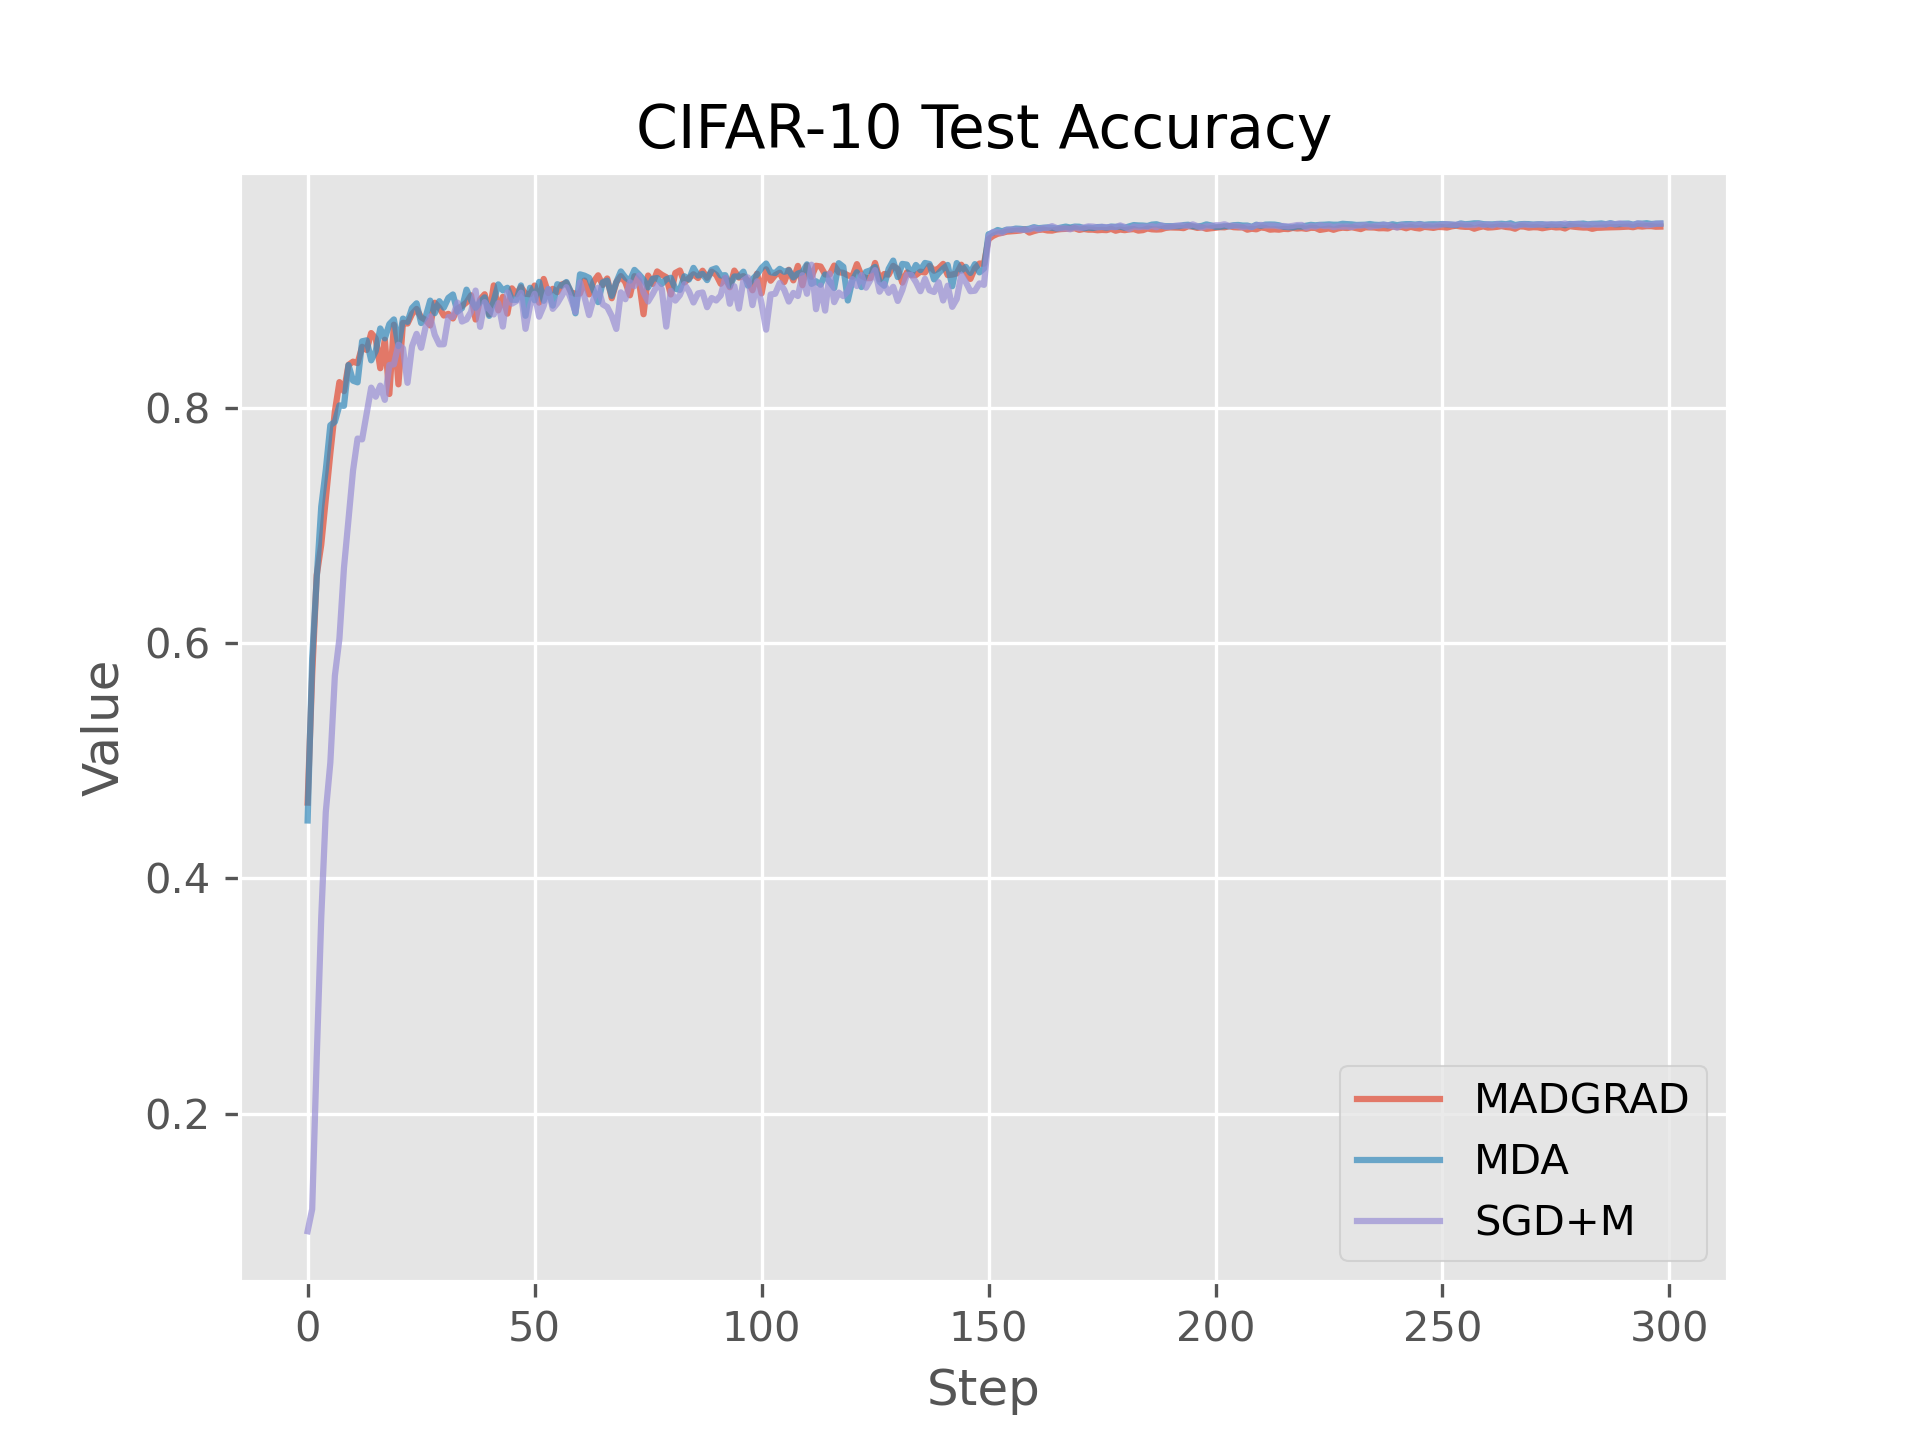
\includegraphics[width=\linewidth]{../ftrl_dl_data/CIFAR-10_test_acc.png}
    \caption{Test Accuracy of Optimizers on CIFAR-10}
    \label{fig:sub1}
  \end{subfigure}%
  \begin{subfigure}{.5\textwidth}
    \centering
    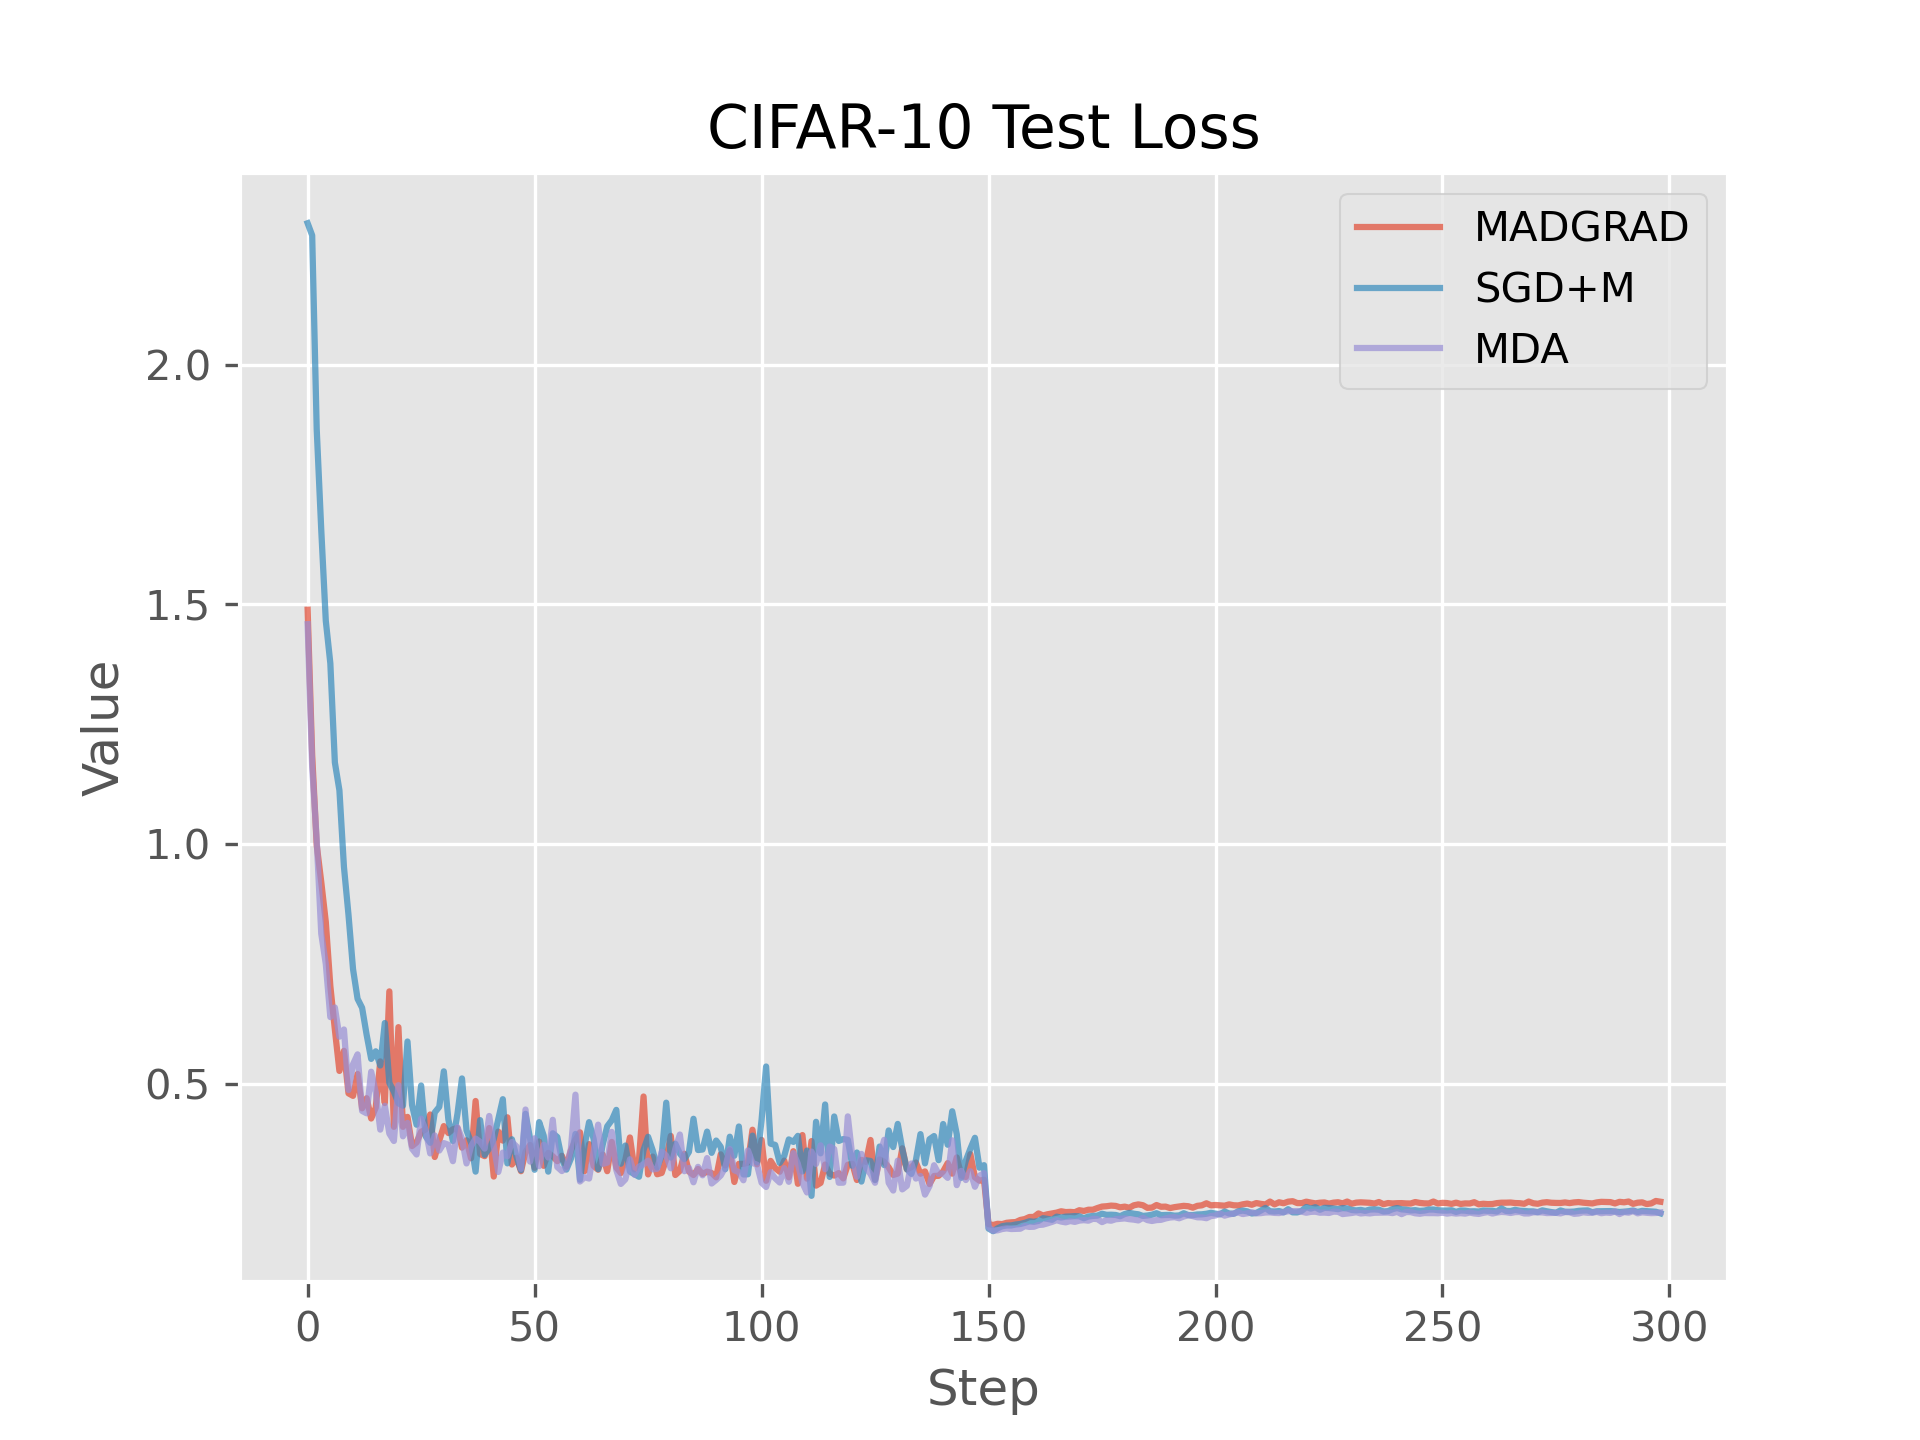
\includegraphics[width=\linewidth]{../ftrl_dl_data/CIFAR-10_test_loss.png}
    \caption{Test Loss of Optimizers on CIFAR-10}
    \label{fig:sub2}
  \end{subfigure}
  \caption{Comparison of optimizer performance on CIFAR-10 dataset}
  \label{fig:test}
\end{figure}

Our experiment setup and optimizer implementations for MDA and MADGRAD can be found at
\url{https://github.com/shashankmanjunath/ftrl_deep_learning}.

\section{Theory}

When proving the convergence bound for MADGRAD, the authors require an alternative definition of
MADGRAD than the one presented in the paper and implemented. In the original MADGRAD algorithm presented in the paper,
the $z_{k+1}$ is given by:

\[
  z_{k+1} = x_0 - \frac{1}{\sqrt[3]{v_{k+1}} + \epsilon} \circ s_{k+1}
\]

where $\circ$ indicates the Hadamard product. $\epsilon$ is included for numerical stability in the early iterations of
the algorithm, as the $v_{k+1}$ parameter can be 0. However, in the convergence proof, the $z_{k+1}$ parameter is given
by:

\[
  z_{k+1} = x_0 - \frac{1}{\sqrt[3]{\lambda_{k+1}G^2 + v_{k+1}}} \circ s_{k+1}
\]

Note the extra $\lambda_{k+1}G^2$ in the denominator, which is used to create the following upper bound leveraged in the
overall convergence proof:

\[
  \sum\limits_{t=0}^k \frac{\lambda_t^2 g_t^2}{\sqrt[3]{\lambda_t G^2 + \sum\limits_{i=0}^{t-1} \lambda_i g_i^2}} \leq
  \frac{3}{2} \lambda_k \left(\sum\limits_{i=1}^k \lambda_i g_i^2\right)^{\frac{2}{3}}
\]

This extra $\lambda_t G^2$ prevents the algorithm from being \emph{scale-free}, or an algorithm that is invariant to the
scaling of losses by a constant factor. Therefore, we aim to construct a convergence proof which maintains the
scale-free nature of the algorithm.

\subsection{Proof of Scale-Free Regret Bound for MADGRAD}

\todo{Talk about assumptions}

Consider the MADGRAD algorithm. This algorithm implements FTRL with the regularizer: 

\[
  \psi_t(\bx) = \frac{1}{2} \|\bx - \bx_0 \|_{A_t}
\]

where $A_t = \diag(\alpha_t)$, and $\alpha_t = \sqrt[3]{\sum\limits_{i=1}^{t-1}\lambda_i g_i^2}$. Note that
$\psi_t(\bx)$ is strongly-convex with respect to the norm $\| \cdot \|_{A_t}$. Let us denote the Bregman divergence of a
function $f$ over two vectors $\bx, \by \in \R^D$ by $B_f(\bx; \by)$ and let $f^\star$ indicate the Fenchel conjugate of
$f$. In order to prove the scale-free bound, we make the reduction that $c_t = 1$ for all rounds. This effectively
removes the momentum operation, and leaves us with only FTRL iterates. Let us first make a useful proposition.

\begin{proposition}[Proposition 2 in \cite{orabona_generalized_2014}: Properties of Fenchel Conjugates of Strongly
  Convex Functions]\label{prop:1}
  Let $K \subseteq V$ be a non-empty closed convex set. Let $\lambda \geq 0$, and let $f: K \rightarrow R$ be a lower
  semi-continuous function that is $\lambda$-strongly convex with respect to $\| \cdot \|$. The Fenchel conjugate of f
  satisfies:

  \begin{enumerate}
    \item $f^*$ is finite everywhere and differentiable
    \item $\nabla f^* (\ell) = \argmin_{w \in K}(f(w) - \langle \ell, w \rangle)$
    \item For any $\ell \in V^*$, $f^*(\ell) + f(\nabla f^*(\ell)) = \langle \ell, \nabla f^\star (\ell) \rangle$
    \item $f^*$ is $\frac{1}{\lambda}$-strongly smooth, i.e. for any $x, y \in V^*$, $B_{f^*}(x, y) \leq
      \frac{1}{2\lambda}\|x - y \|_*$
    \item $f^*$ has $\frac{1}{\lambda}$-Lipschitz continuous gradients, i.e. $\| \nabla f^*(x) - \nabla f^*(y)\| \leq
      \frac{1}{\lambda}\|x - y\|_*$ for any $x, y \in V^*$
  \end{enumerate}
\end{proposition}

Let us now define some useful lemmas.

\begin{lemma}[Lemma 1 in \cite{orabona_generalized_2014}] \label{lemma:1}
  Let $\{\psi_t\}_{t=1}^\infty$ be a sequence of functions defined on a common convex domain $S \subseteq \R^n$ and
  such that each $\psi_t$ is $\mu_t$-strongly convex with respect to the norm $\|\cdot\|_t$. Let $\|\cdot\|_{t, \star}$ be
  the dual norm of $\| \cdot \|_t$, for $t = 1, 2, \cdots, T$. Then, for any $\bu \in S$,

  \[
    \Regret _T (\bu) \leq \sum\limits_{t=1}^T \langle g_t, \bu - \bx_t \rangle \leq \psi_{T}(\bu) + \psi_{1}^\star (0) +
    \sum\limits_{t=1}^T B_{\psi_{t}^\star}(-\theta_t, -\theta_{t-1}) - \psi_{t}^\star (-\theta_t) +
    \psi_{t+1}^\star(-\theta_t)
  \]
\end{lemma}

\proof Given in (\cite{orabona_generalized_2014})
\qed

\begin{lemma} \label{lemma:2}
  Let $a_1, a_2, \cdots, a_t$ be non-negative real numbers. If $a_1 > 0$, then
  \[
    \sum\limits_{t=1}^T \frac{a_t}{\sqrt[3]{\sum\limits_{s=1}^t a_s}} \leq \frac{3}{2}\left(\sum\limits_{t=1}^T
    a_t\right)^\frac{2}{3}
  \]
\end{lemma}

\proof Note that if $0 \leq x \leq 1$, 

\[
  \frac{2}{3} x \leq 1 - (1 - x)^\frac{2}{3}
\]

Let $L_t = \sum\limits_{i=1}^t \ell_i$, and let $x = \frac{\ell_t}{L_t}$. Let $\ell_0 = 0$.

\begin{align*}
  \frac{2}{3} \frac{\ell_t}{L_t}
  &\leq 1 - (1 - \frac{\ell_t}{L_t})^\frac{2}{3} = 1 - (\frac{L_{t-1}}{L_t})^\frac{2}{3} \\
  \frac{2}{3} \frac{\ell_t}{L_t} L_{t}^\frac{2}{3} &\leq L_{t}^\frac{2}{3} - L_{t-1}^\frac{2}{3} \\
  \frac{2}{3} \frac{\ell_t}{\sqrt[3]{L_t}} &\leq L_{t}^\frac{2}{3} - L_{t-1}^\frac{2}{3} \\
  \therefore \frac{2}{3} \sum\limits_{t=1}^T \frac{\ell_t}{\sqrt[3]{L_t}} &\leq \sum\limits_{t=1}^T L_{t}^\frac{2}{3} -
  L_{t-1}^\frac{2}{3} \\
  \sum\limits_{t=1}^T \frac{\ell_t}{\sqrt[3]{L_t}} &\leq \frac{3}{2} L_{T}^\frac{3}{2} \\
  \sum\limits_{t=1}^T \frac{\ell_t}{\sqrt[3]{L_t}} &\leq \frac{3}{2} \left(\sum\limits_{t=1}^T \ell_t \right)^\frac{2}{3}
\end{align*}

Letting $\ell_i = a_i \forall i$ yields the lemma.

\qed

\begin{lemma} \label{lemma:3}
  Let $C, a_1, a_2, \cdots, a_T \geq 0$, and $\alpha \geq 1, \alpha \neq \min\limits_{t=1,2,\cdots,T}a_{t}^\frac{4}{3}$.
  Then,

  \[
    \sum\limits_{t=1}^T \min \left\{ \frac{a_{t}^2}{\sqrt[3]{\sum\limits_{s=1}^{t-1} a_{s}^2}}, C a_t\right\} \leq
    \frac{C \alpha}{\alpha - \min\limits_{t=1,2,\cdots,T}a_{t}^\frac{4}{3}} \max\limits_{t=1,2,\cdots,T} a_t
    + 2\sqrt[3]{1 + \alpha^2} \sqrt{\sum\limits_{s=1}^T a_{s}^3}
  \]
\end{lemma}

\proof We will prove this bound by proving each individual case in the minimum, then summing them.

\emph{Case 1}. Consider $a_t \leq \alpha^3 \left(\sum\limits_{s=1}^{t-1} a_s^2\right)^\frac{2}{3}$.

\begin{align*}
  \min \left\{ \frac{a_{t}^2}{\sqrt[3]{\sum\limits_{s=1}^{t-1} a_{s}^2}}, C a_t \right\} 
  &\leq \frac{\alpha_{t}^2}{\sqrt[3]{\sum\limits_{s=1}^{t-1}a_{s}^2}} =
  \frac{a_{t}^2}{\sqrt[3]{\frac{1}{1+\alpha^2}\left(\alpha^2 \sum\limits_{s=1}^{t-1} a_{s}^2 +
  \sum\limits_{s=1}^{t-1} a_{s}^2 \right)}} \\
  &\leq \frac{a_{t}^2 \sqrt[3]{1 + \alpha^2}}{\sqrt[3]{a_{t}^2 + \sum\limits_{s=1}^{t-1} a_{s}^2}} = \frac{a_{t}^2
  \sqrt[3]{1 + \alpha^2}}{\sqrt[3]{\sum\limits_{s=1}^t a_{s}^2}}
\end{align*}

Note that $\frac{x^2}{\sqrt[3]{x^2 + y^2}} \leq 2(\sqrt{x^3 + y^3} - \sqrt{y^3})$. Using this inequality,

\[
  \sqrt[3]{1 + \alpha^2} \frac{a_{t}^2}{\sqrt[3]{\sum\limits_{s=1}^t a_{s}^2}} \leq 2 \sqrt[3]{1 +
  \alpha^2}\left(\sqrt{\sum\limits_{s=1}^t a_{s}^3} - \sqrt{\sum\limits_{s=1}^{t-1} a_{s}^3}\right)
\]

\emph{Case 2} Consider $a_{t}^2 \geq \alpha^3 \left(\sum\limits_{s=1}^{t-1} a_{s}^2\right)^\frac{2}{3}$. Note that this
implies that $a_t \geq \alpha^\frac{3}{2} \sqrt[3]{\sum\limits_{s=1}^{t-1} a_{s}^2}$. Additionally, let 
$A = \left( \sum\limits_{s=1}^{t-1} a_{s}^2 \right)^\frac{2}{3}$.


\begin{align*}
  \min \left\{ \frac{a_{t}^2}{\sqrt[3]{\sum\limits_{s=1}^{t-1} a_{s}^2}}, C a_t \right\}
  &\leq C a_t = C a_t \left(\frac{\alpha - A}{\alpha -A}\right) \\
  &\leq \frac{C}{\alpha - A}\left(\alpha a_t - A a_t\right) = \frac{C \alpha}{\alpha - A}\left(a_t - \alpha^\frac{1}{2}
    A \sqrt[3]{\sum\limits_{s=1}^{t-1} a_{s}^2}\right) \\
  &\leq \frac{C \alpha}{\alpha - A}\left(a_t - \left( \sum\limits_{s=1}^{t-1} a_{s}^2 \right)^\frac{2}{3}
  \left(\sum\limits_{s=1}^{t-1} a_{s}^2\right)^\frac{1}{3}\right) \\
  &\leq \frac{C \alpha}{\alpha - A}\left(a_t - \sqrt{\sum\limits_{s=1}^{t-1} a_{s}^2}\right)
\end{align*}

Let $M_t = \max \{a_t, \cdots, a_t\}$. Note that in this case, $a_t = M_t$, and $\sqrt{\sum\limits_{s=1}^{t-1} a_{s}^2}
\geq M_{t-1}$. Therefore,

\[
  \min \left\{ \frac{a_{t}^2}{\sqrt[3]{\sum\limits_{s=1}^{t-1} a_{s}^2}}, C a_t \right\} \leq 
  \frac{C \alpha}{\alpha - A}\left(M_t - M_{t-1}\right)
\]

Further note that since $a_t \geq 0 \forall t$, $A = (\sum\limits_{s=1}^T a_{s}^2)^\frac{2}{3} \geq
\min_{t=1,\cdots,T}a_{t}^\frac{4}{3}$. Let $B = \min_{t=1,\cdots,T}a_{t}^\frac{4}{3}$, Therefore,

\[
  \min \left\{ \frac{a_{t}^2}{\sqrt[3]{\sum\limits_{s=1}^{t-1} a_{s}^2}}, C a_t \right\} \leq 
  \frac{C \alpha}{\alpha - B}\left(M_t - M_{t-1}\right)
\]

Therefore, combining the two cases, we have:

\[
  \min \left\{ \frac{a_{t}^2}{\sqrt[3]{\sum\limits_{s=1}^{t-1} a_{s}^2}}, C a_t \right\} \leq \frac{C \alpha}{\alpha -
  B}\left(M_t - M_{t-1}\right) + 2 \sqrt[3]{1 + \alpha^2}\left(\sqrt{\sum\limits_{s=1}^t a_{s}^3} -
  \sqrt{\sum\limits_{s=1}^{t-1} a_{s}^3}\right)
\]

Therefore, summing from $t=1$ to $T$,

\[
  \sum\limits_{t=1}^T\min \left\{ \frac{a_{t}^2}{\sqrt[3]{\sum\limits_{s=1}^{t-1} a_{s}^2}}, C a_t \right\} \leq \frac{C
  \alpha}{\alpha - B}\left(\max\limits_{t=1, \cdots, T} a_t\right) + 2 \sqrt[3]{1 +
  \alpha^2}\left(\sqrt{\sum\limits_{t=1}^T a_{t}^3}\right)
\]

\qed

Let us now state the overall convergence bound for our version of MADGRAD.

\begin{theorem} \label{theorem:1}
  Suppose $K \subseteq \R^D$ is a non-empty closed convex subset. Suppose that a regularizer $\psi_t: K \rightarrow \R$
  is a non-negative lower semi-continuous function that is $\mu_t$ strongly convex with respect to a norm $\| \cdot
  \|_t$. The regret of non-momentumized MADGRAD satisfies:

  \begin{align*}
    \Regret_T(u) \leq \sum\limits_{d=1}^D \frac{\psi_d(u_d)}{\sqrt[3]{\sum\limits_{i=1}^{T} \lambda_i
      g_{id}^2}} + \frac{3}{2}\left(\sum\limits_{t=1}^T \lambda_t g_{td}^2\right)^\frac{2}{3} +& \frac{2
      \sqrt{T-1}\left(\sum_{i=1}^{t-1} \lambda_i g_{id}^2\right)}{1 - \left( \sum_{i=1}^{t-1} a_{i}^2
    \right)^\frac{2}{3}} \max_{t \leq T} \sqrt{\lambda_t}|g_{td}| \\ &+ 2\sqrt[3]{2}\sqrt{\sum\limits_{t-1}^T
    \lambda_t^\frac{3}{2} |g_{td}|^3}
  \end{align*}
\end{theorem}

\proof Note that $\psi_t (x) = \frac{1}{2} \| \bx - \bx_0\|_{A_t}^2$, where $A_t = \diag(\alpha_t)$. For this
regularizer, $\alpha_t = \sqrt[3]{\sum\limits_{i=1}^{t-1} \lambda_i g_{i}^2} \in \R^D$. Let $L_t = \sum\limits_{i=1}^t
\lambda_i g_i$.Let us perform this analysis per-coordinate.

\[
  \psi_{t,d}(\bx) = \frac{1}{2} (\bx_d - \bx_{0,d})\sqrt[3]{\sum\limits_{i=1}^{t-1} \lambda_i g_{id}^2}(\bx_d -
  \bx_{0,d}) = \frac{1}{2}\sqrt[3]{\sum\limits_{i=1}^{t-1} \lambda_i g_{id}^2}(\bx_d - \bx_{0,d})^2.
\]

Let $\eta_{t,d} = \frac{1}{\sqrt[3]{\sum\limits_{i=1}^{t-1} \lambda_i g_{id}^2}}$. Therefore, we have:

\begin{align*}
  \psi_{t,d} (\bx) &= \frac{1}{\eta_{t,d}} \psi_d(\bx) \\
  \psi_d(\bx) &= \frac{1}{2} (\bx_d - \bx_{0,d})
\end{align*}

Since $A_t$ is a diagonal matrix, $\psi_t(\bx)$ is $\min\limits_{D} \sqrt[3]{\sum\limits_{i=1}^{t-1} \lambda_i
g_{i}^2}$-strongly convex. We can tighten this bound by analyzing $\psi_{t,d}(\bx)$ and establishing a per-coordinate
strong convexity bound. Recall that, since $\psi_d(\bx): \R \rightarrow \R$, we can find the strong convexity by finding
the lower bound of the second derivative of $\psi_d(\bx)$.

\begin{align*}
  \frac{d \psi_d(\bx)}{d \bx_d} &= \bx_d - \bx_{0,d} \\
  \frac{d^2 \psi_d(\bx)}{d \bx_d^2} &= 1
\end{align*}

Therefore, $\psi_d(\bx)$ is 1-strongly convex with respect to $| \cdot |$, as we are dealing with real numbers in the
per-coordinate case. By Lemma 1, we have:

\[
  \Regret_T(\bu) \leq \psi_{T+1}(\bu) + \psi_{1}^\star (\textbf{0}) + \sum\limits_{t=1}^T B_{\psi_{t}^\star}(-L_t,
  -L{t-1}) - \psi_{t}^\star (-L_t) + \psi_{t-1}^\star(-L_t)
\]

Writing this in a per-coordinate manner,

\begin{align*}
  \Regret_T(\bu) 
  &\leq \sum\limits_{d=1}^D \psi_{T+1,d}(\bu) + \psi_{1,d}^\star (\textbf{0}) + \sum\limits_{t=1}^T
  B_{\psi_{t,d}^\star}(-L_t, -L{t-1}) - \psi_{t,d}^\star (-L_t) + \psi_{t-1,d}^\star(-L_t) \\
  &\leq \sum\limits_{d=1}^D \frac{1}{\eta_{T+1}}\psi_{d}(\bu) + \frac{1}{\eta_1}\psi_{d}^\star (\textbf{0}) + \sum\limits_{t=1}^T
  B_{\psi_{t,d}^\star}(-L_t, -L{t-1}) - \psi_{t,d}^\star (-L_t) + \psi_{t-1,d}^\star(-L_t)
\end{align*}

Let us proceed by bounding $B_{\psi_{t,d}^\star}(-L_t, -L{t-1}) - \psi_{t,d}^\star (-L_t) + \psi_{t-1,d}^\star(-L_t)$ in
two ways.

\begin{enumerate}
  \item By Proposition \ref{prop:1} item 4, we know that $B_{\psi_{t,d}^*}(-L_t, -L_{t-1}) \leq \frac{\eta_t \lambda_t
    g_{t,d}^2}{2 \mu_{t,d}} = \frac{\eta_t \lambda_t g_{t,d}^2}{2}$. Therefore, by Lemma \ref{lemma:1}, we know that:

    \[
      B_{\psi_{t,d}^*)}(-L_t, -L_{t-1}) - \psi_{t,d}^*(-L_t) + \psi_{t+1,d}^*(-L_t) \leq B_{\psi_{t,d}^*}(-L_t,
      -L_{t-1}) \leq \frac{\eta_t \lambda_t g_{t,d}^2}{2}
    \]

    \todo{since $\psi_{t,d}^* \geq \psi_{t+1,d}^*$}.
  \item Similarly,

    \begin{align*}
      B_{\psi_{t,d}^*}(-L_t, -L_{t-1}) 
      &- \psi_{t,d}^*(-L_t) + \psi_{t+1,d}^*(-L_t) = B_{\psi_{t+1,d}^*}(-L_t, -L_{t-1}) + \psi_{t+1,d}^*(-L_{t-1}) \\
      & - \psi_{t,d}^*(-L_{t-1}) + \langle \nabla \psi_{t,d}^*(-L_{t-1}) - \nabla \psi_{t+1,d}^*(-L_{t-1},
      g_{t,d}))\rangle \\
      &\leq \frac{1}{2} \eta_{t+1,d}\lambda_t g_{t,d}^2 + | \nabla \psi_{t,d}^*(-L_{t-1}) - \nabla
      \psi_{t+1,d}^*(-L_{t-1})| |g_{t,d}| \\
      &\leq \frac{1}{2} \eta_{t+1,d}\lambda_t g_{t,d}^2 + | \nabla \psi_{d}^*(-\eta_{t,d} L_{t-1}) - \nabla
      \psi_{d}^*(-\eta_{t+1}L_{t-1})| |g_{t,d}| \\
      &\leq \frac{1}{2} \eta_{t+1,d}\lambda_t g_{t,d}^2 + |L_{t-1}|(\eta_{t,d} - \eta_{t+1,d})|g_{t,d}|
    \end{align*}

    Recall that $\eta_{t,d} = \frac{1}{\sqrt[3]{\sum\limits_{i=1}^{t-1} \lambda_i g_{id}^2}}$. Therefore,

    \begin{align*}
      |L_{t-1}|(\eta_{t,d} - \eta_{t+1,d}) 
      &\leq |L_{t-1}|\eta_{t,d} = \frac{\sum_{i=1}^{t-1} \lambda_i g_{i,d}}{\sqrt[3]{\sum_{i=1}^{t-1}\lambda_i
      g_{i,d}^2}} \\
      &\leq \frac{\sqrt{(\sum_{i=1}^{t-1} \sqrt{\lambda_i} g_{i,d}
      \sqrt{\lambda_i})^2}}{\sqrt[3]{\sum_{i=1}^{t-1} \lambda_i g_{i,d}^2}} \\
      &\leq \frac{\sqrt{(\sum_{i=1}^{t-1} \lambda_i)(\sum_{i=1}^{t-1}\lambda_i g_{i,d}^2)}}{\sqrt[3]{\sum_{i=1}^{t-1} \lambda_i g_{i,d}^2}}
    \end{align*}

    By Callebaut's inequality. Therefore, we have:

    \[
      |L_{t-1}|(\eta_{t,d} - \eta_{t+1,d}) \leq \left(\sqrt{\sum_{i=1}^{t-1} \lambda_i}\right)\left(\sum_{i=1}^{t-1}\lambda_i
      g_{i,d}^2\right)^\frac{2}{3}
    \]
\end{enumerate}

Combining these two bounds, we have:

\[
  B_{\psi_{t,d}^*}(-L_t, -L_{t-1}) - \psi_{t,d}^*(-L_t) + \psi_{t+1,d}^*(-L_t) \leq \frac{\eta_t \lambda_t g_{t,d}^2}{2}
  + \left(\sqrt{\sum_{i=1}^{t-1} \lambda_i}\right)\left(\sum_{i=1}^{t-1}\lambda_i g_{i,d}^2\right)^\frac{2}{3}
\]

Note that 
\[
  \sqrt{\sum\limits_{i=1}^{t-1}\lambda_i} \leq \sqrt{(t-1) \lambda_t} = \sqrt{t-1}\sqrt{\lambda_t}
\]

Let $H = \left(\sum\limits_{i=1}^{t-1} \lambda_i g_{i,d}^2\right)^\frac{2}{3} \sqrt{t-1}$. Therefore, we have:

\[
  B_{\psi_{t,d}^*}(-L_{t}, -L_{t-1}) - \psi_{t,d}^*(-L_t) + \psi_{t+1,d}^*(-L_t) \leq \frac{\eta_{t+1,d} \lambda_t
  g_{t,d}^2}{2} + H \sqrt{\lambda_t}|g_{t,d}|
\]

Therefore, we have an overall regret bound of

\begin{align}
  \Regret_T(\bu) 
  &\leq \sum\limits_{d=1}^D \frac{1}{\eta_{T+1}}\psi_{d}(\bu) + \frac{1}{\eta_1}\psi_{d}^*(0)+\sum\limits_{t=1}^T \min
  \left\{\frac{\eta_t \lambda_t g_{t,d}^2}{2}, \frac{\eta_{t+1,d} \lambda_t g_{t,d}^2}{2} + H
  \sqrt{\lambda_t}|g_{t,d}|\right\} \nonumber \\
  \therefore \Regret_T(\bu) 
  &\leq \frac{1}{\eta_{T+1}}\psi_{d}(\bu) + \frac{1}{\eta_1}\psi_{d}^*(0)+\frac{1}{2}\sum\limits_{t=1}^T \eta_{t+1}
  \lambda_t g_{t,d}^2 + \frac{1}{2}\sum\limits_{t=1}^T \min \left\{\frac{\eta_t \lambda_t g_{t,d}^2}{2},  2H
  \sqrt{\lambda_t}|g_{t,d}|\right\} \label{eq:1}
\end{align}

Let us bound this regret in three groups.

\begin{enumerate}
\item $\frac{1}{2}\sum\limits_{t=1}^T \min \left\{\frac{\eta_t \lambda_t g_{t,d}^2}{2}, 2H\sqrt{\lambda_t}|g_{t,d}|\right\}$

  We bound this using Lemma \ref{lemma:3}. Let $B = \min_{t\leq T}a_{t}^\frac{4}{3}$ setting $\alpha = 1+B$.
  \[
    \frac{1}{2}\sum\limits_{t=1}^T \min \left\{\frac{\eta_t \lambda_t g_{t,d}^2}{2}, 2H\sqrt{\lambda_t}|g_{t,d}|\right\}
    \leq 2H(1+B)\max_{t\leq T}\sqrt{\lambda_t}|g_{t,d}| +
    2\sqrt[3]{1 + (1+B)^2}\sqrt{\sum\limits_{t=1}^T \lambda_{t}^\frac{3}{2} g_{t,d}^3}
  \]
\item $\sum\limits_{t=1}^T \frac{\lambda_t g_{t,d}^2}{\sqrt[3]{\sum\limits_{i=1}^t}\lambda_i g_{i,d}^2}$. We bound this
  by Lemma \ref{lemma:2}.

  \[
    \sum\limits_{t=1}^T \frac{\lambda_t g_{t,d}^2}{\sqrt[3]{\sum\limits_{i=1}^t\lambda_i g_{i,d}^2}} \leq \frac{3}{2}
    \left(\sum\limits_{t=1}^T \lambda_t g_{t,d}^2\right)^\frac{2}{3}
  \]
\item $\frac{1}{\eta_{T+1}}\psi_{d}(\bu) + \frac{1}{\eta_1}\psi_{d}^*(0)$.

  Note that $\psi_d(\bu) = \frac{1}{2}(\bu_d - x_{0,d})$. Therefore,

  \[
    \frac{1}{\eta_{T+1,d}}\psi_d(\bu) = \frac{(\bu_d - x_{0,d})^2}{2 \sqrt[3]{\sum\limits_{t=1}^T \lambda_i g_{i,d}^2}}
  \]

  Now let us analyze $\psi_d^*(0)$. By Proposition \ref{prop:1} item 2,

  \begin{align*}
    \psi_d^*(0) = \sup\limits_{x \in K}(\langle x , 0 \rangle - \psi_d(x)) = \sup_{x \in K}(-\frac{1}{2}(\bx_d -
    x_{0,d})) \leq 0
  \end{align*}

  Therefore, $\frac{1}{\eta_{T+1}}\psi_{d}(\bu) + \frac{1}{\eta_1}\psi_{d}^*(0) \leq \frac{1}{\eta_{T+1}}\psi_{d}(\bu)$
\end{enumerate}

Substituting these three upper bounds back into (\ref{eq:1}) gives the desired bound. \\
\qed

\bibliographystyle{plainnat}
\bibliography{project_report}

\end{document}
